

\documentclass[eng]{ajceam-class}
%
% Publication Title
\title{Convolución y deconvolución de imágenes con métodos ciegos y no ciegos}

% Publication Title (Portuguese only)
\titulo{Poner aquí el titulo del proyecto}

% Short title for the header (copy the main title if it is not too long)
% 
       
% Authors
\author[1]{Adara L Pulido Sánchez}
\author[2]{Guillermo Villegas Morales}
%\author[1,2,3]{Name C. Surname}

% Author Affiliations
\affil[1]{Tecnologico de Monterrey, Escuela de Ingenieria y Ciencias}
%\affil[2]{(Other) University Name, Department Name or Institute, State, Country}
%\affil[3]{(Other) University Name, Department Name or Institute, State, Country}


% Surname of the first author of the manuscript
\firstauthor{Adara Pulido-Sánchez and Guillermo Villegas}

%Contact Author Information
\contactauthor{Name A. Surname}           % Name and surname of the contact author
\email{name.surname@email.com}            % Contact Author Email

% Publication data (will be defined in the edition)
\thisvolume{XX}
\thisnumber{XX}
\thismonth{Month}
\thisyear{20XX}
\receptiondate{24/11/203}


% Place your particular definitions here
\newcommand{\vect}[1]{\mathbf{#1}}  % vectors

% Insert here the abstract in English language
\abstract{
Now a days video surveillance systems are of big importance to many cities. It is quite common to find devices with a poor-quality output, this makes many video devices unable to provide relevant information and solve the problems they are supposed to. Two methods to improve the quality of images captured by security cameras are discussed in this article: blind and non-blind convolution and deconvolution. For both methods mathematical methods such as the fast Fourier transform (FFT), Gaussian filter, point spread function (PSF), amongst others were used. With both methods significant improvements in image quality were obtained, being the non-blind convolution and deconvolution method the most effective. This method presented remarkable improvements. While non-blind convolution and deconvolution, despite being the most interesting in most contexts, had slightly inferior results, however the product is still a good improvement over an image with a convolution. Both methods present useful results and are very promising in the image processing field.
%This document provides a template for the preparation of original work whose authors wish to %be published in the Academic Journal on Computing, Engineering and Applied Mathematics of the %Universidade Federal do Tocantins Tocantins, Brazil. At first, we strongly recommend the %summary to be written as a single paragraph containing at least 150 and at most 200 words. In %this text section, it is expected a summary including the context, motivation, methodology, %the most original contributions, results, and conclusions of your work. In addition, %bibliographic citations, acronyms, or formulas should be avoided in the abstract as well as in %the title. It is also strongly recommended to avoid any references to figures or tables in %this section. Finally, it is a good practice to write your article by inserting text to and %deleting from straight to/from this template file in order to maintain the predefined styles.
}
%Abstrac no debe tener ejemplos, citas ni aclaraciones, se hace hasta el final, esta en ingles, voz pasiva, la primera frase debe ser importante.

% Insert here the keywords of your work in English language
\keywords{
convolución de imágenes, deconvolución ciega, PSF, filtro Guassiano, operador Sobel, transformada de Fourier}



% Start document
\begin{document}

% Include title, authors, abstract, etc.
\maketitle
\thispagestyle{fancy}


% Main body of manuscript
\section{Introduction}
\firstword{E}{n}% Capital letter in first word
el mundo actual, donde los sistemas de comunicación se encuentran altamente desarrollados y la interconectividad forma parte de la vida cotidiana en la mayoría de las ciudades del planeta es muy común encontrar sistemas cerrados de videovigilancia, la mayoría  de ellos instalados por los propios usuarios bajo la necesidad de proteger sus espacios y muchos de ellos con no muy buena calidad de imagen, pero sí buscando cubrir con lo básico tal vez incluso para solamente desanimar a los delincuentes.

 La utilización de cámaras de videovigilancia son parte de una política pública de prevención del delito, cuyo objetivo principal es reducir la oportunidad para los que transgreden la ley así como para maximizar la oportunidad de responsabilizar al culpable. 
 Cada vez más personas invierten en tecnología tanto como para prevención o como reacción a un delito previo. En muchas ocasiones se invierte de lo que se dispone, es decir no todos los sistemas cuentan con un alto presupuesto, por lo que se recurre a tecnología de más bajo costo; es entonces cuando los resultados de la imagen suelen presentar baja calidad debido a la resolución y compresión del archivo , la forma en que se graba y el recorte que generalmente ocurre en dichos archivos de video. La mayoría de las imágenes de los sistemas de video seguridad son pixeles, mejorar estas  imágenes implica utilizar software especializado para la recuperación de la imagen. 

 Debido a la inversión que hacen gobiernos y sociedad  ahora es más común  encontrar evidencia en video sobre muchísimas situaciones que ameritan seguimiento ya sea legal, social o simplemente de identificación, lo importante es que esa información sea nítida para que pueda utilizarse adecuadamente.

 Para resolver este problema, se partirá de la idea de que el desenfoque presetado en la imagen observada se debe a la Función de Dispersión de Puntual PSF (Point Spread Function), el cual se describe como la imagen bidimensional de un punto en el espacio objeto. Para esto se parte de se parte de la ecuacion $g(x)=F(x)h(x)$, en donde $F(x)$ es la imagen original sin desenfoque, $h(x)$ es el kernel de desenfoque (PSF), mientras que $g(x)$ es la imagen observada. 
 
\section{Metodología}


    \textbf{Transformada de Fourier}

La transfomarda de Fourier proporciona un modo para definir el concepto relacionado de escala de frecuencia de una señal periódica, puesto que permite una descomposición única de las señales. Se basa en el uso de funciones de base sinosoidal y solo tiene resolución de frecuencia, es decir ninguna de tiempo según como se declara en \cite{Filchev2020}. Dentro de las Transformadas de Fourier a utilizar se encuentra la transformada discreta de Fourier es de suma importancia en el ámbito de procesamiento de señal digital, puesto que se usa para derivar la representación de un dominio de frecuencia de señal. \cite{Giannakopoulos2014} La transformada discreta de Fourier es un producto matriz vector, el cual se le conoce como vector de las muestras de entrada a $(x_{0},w_{1},...x_{N-1})^T$. Esta definido como:

\begin{equation} \label{ec-1}
 F(k)=\sum_{n=0}^{N-1} f(n) \exp{-j\frac{2\pi}{N}kn}, k=0,...,N-1
\end{equation}

Por otro lado, tambien esta la transformada rapida de Fourier (FFT) la cual en convolución parte de la multiplicación del dominio de la frecuencia, corresponde a la convolución en el dominio del tiempo. Posteriormente se transforma la señal de entrada en el dominio de frecuencia mediante la transformada discreta de Fourier, la cual se multiplica por la respuesta de frecuencia del filtro para luego transformarse nuevamente al dominio del tiempo por medio de la transformada discreta inversa de Fourier \cite{Smith2003}.

\textbf{Convolución}


La convolución se describe como la función equivalente a la integral o la sumatoria de dos funciones componentes, lo que mide la superposición cuando una función se desplaza sobre otra. Este proceso implica la inversión con respecto de la variable independiente de una de las funciones, para posteriormente desplazarla con el cambio de la variable  $t$ a $\tau$. Sean $f$ y $g$ funciones en $t$, entonces la convolución de ambas en un intervalo infinito esta dada por la integral\cite{kim2013applications}:

\begin{equation} \label{ec-1}
 f*g \equiv \int_{-\infty}^{\infty} f(\tau)g(t-\tau) d\tau
\end{equation}

En cambio cuando la convolución se realiza en un intervalo finito en un rango $[0,t]$ se expresa como:

\begin{equation} \label{ec-2}
 [f*g](t) \equiv \int_{0}^{t} f(\tau)g(t-\tau) d\tau
\end{equation}

\textbf{Teorema de convolución}

 Para simplificar este proceso, haremos uso del teorema de convolución, el cual establece que si se tienen dos funciones $f$ y $g$ con transformadas de Fourier, entonces la convolución de ambas funciones en el espacio real es igual al producto de sus transformadas de Fourier en el espacio de Fourier. 

\begin{equation} \label{ec-3}
    f(r) \ast \ast g(r) \longleftrightarrow F(k)G(k)
\end{equation}

Otra forma de esta expresión está dada por 
\begin{equation}\label{ec-4}
    f \ast g = \alpha F\omega G\omega
\end{equation}
donde $\alpha$ es un factor de escala, $F(\omega)$ y $G(\omega)$ son las tranformadas de Fourier de $f$ y $g$ respectivamente.\cite{Jauregui2014}\cite{Blackledge2005} 

\textbf{PSF} 

En el proceso de filtrado de imagenes es necesario conocer conocer la respuesta a un sistema de impulso unitario $\delta(x,y)$, lo cual es equivalente a una celda brillante sobre un fondo homogeneo negro. La Función de Dispersión de Puntual PSF define la respuesta al impulso unitario y se explica como el producto ordenado de dos funciones de dispersión lineal ortogonales.(referencia). La PSF se puede entender como el grado en el que se esparce un punto de luz, esta puede resultar de la tranformada inversa de Fourier de una función de transferencia óptica. \cite{article}


\textbf{Filtro gaussiano} 

La PSF puede tomar diferentes valores según como queramos modelarla, una psf común es el filtro Gaussiano, el cual actúa como un filtro de paso-bajo. Al aplicar este filtro sobre una imagen el producto atenúa las frecuencuas altas y resulta en un efecto de desenfoque. El filtro Gaussiano lo podemos modelar a partir de un parámetro $\partial$ representado una desviación estandar y la función Gaussiana, su PSF está dada por 

\begin{equation}
    h(x,y) = \exp{-\frac{x^2+y^2}{2\partial ^2}}
\end{equation}

Como haremos uso del teorema de convolución para ahorrar recursos computacionales en los procesos de degradación y restauración de imágenes, necesitamos la transformada de Fourier del filtro Gaussiano, este puede ser re-escrito en el dominio de frecuencias como
\begin{equation}
    H(U,V) = \sqrt{2\Pi \partial}e^{-\frac{x^2+y^2}{2\frac{1}{\delta^2}}}
\end{equation}

Como al aplicar este filtro nos da un efecto de una fotografía fuera de foco, es un buen comienzo de estimación de PFS para la deconvolución ciega de una imagen que parezca fuera de foco. \cite{Menaka_2021}

\begin{figure}[!h] 
 \centering
 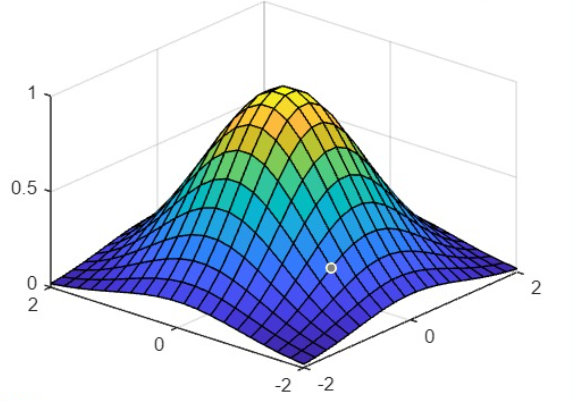
\includegraphics[width=.8\columnwidth]{filtro gaussiano.png} 
 \caption{Representación 3D de un filtro Gaussiano de tamaño 20x20 y desviación estandar de 1} \label{fig-1}
\end{figure}

\textbf {Convolución y deconvolución en imágenes}
    
Ya que tenemos entendido el proceso de convolución en funciones, podemos plantearlo en el contexto de procesamiento de imágenes. El concepto parte de la convolución entre una imagen y una PFS, después podemos o no añadir ruido según el planteamiento. Para simplificar la operación, pasamos las funciones al dominio de frecuencia para convertir la convolución en un producto de dos transformadas de Fourier. A este resultado le aplicamos una transformada de Fourier inversa para obtener una imagen modificada según el filtro inicial. En este caso que aplicamos un filtro Gaussiano, los valores de los píxeles se promediarán entre su vecindad, visualmente se traduce en una imagen borrosa o suavizada. 

Ahora que tenemos nuestra imagen borrosa, si buscamos regresar a la imagen original, podemos simplemente aplicar un filtro inverso, un proceso de deconvolución iterativo o usar algún método de deconvolución ciega. Los primeros dos métodos requieren que tengamos conocimiento o una apuesta de la PFS que degradó a la imagen orginal, mientras que el segundo parte de una PFS arbitraria y busca estimar la PFS óptima para la deconvolución. En cuanto al filtro inverso, si partimos de la ecuación que convoluciona las transformadas de Fourier

\begin{equation}
    B(\omega) = F(\omega)G(\omega)
\end{equation}

Como $B(\omega)$ es la imagen con el filtro aplicado, podemos despejar la imagen original $F(\omega)$ de tal forma que la división entre la imagen filtrada y el filtro nos regrese la imagen original


\begin{equation}
    \frac{B(\omega)}{G(\omega)} = F(\omega)
\end{equation}   

Como todo esto está trabajado en el dominio de las frecuencias, al aplicar la transformada inversa de Fourier obtendremos la imagen inicial percibida. (github)

\begin{figure}[!h] 
 \centering
 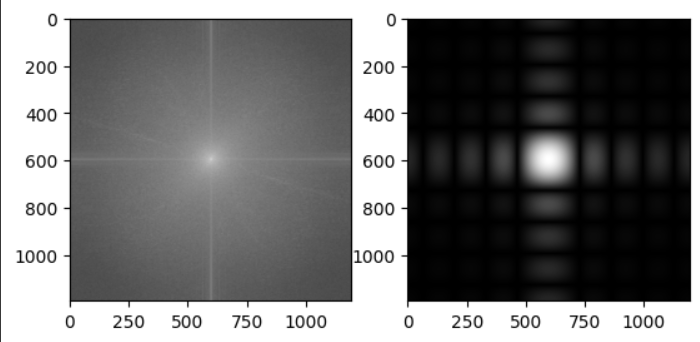
\includegraphics[width=.8\columnwidth]{transformaciones.png} 
 \caption{Tranformaciones de fourier de imagen original (izquierda) y el filtro Gaussiano (derecha)} \label{fig-1}
\end{figure}

\begin{figure}[!h] 
 \centering
 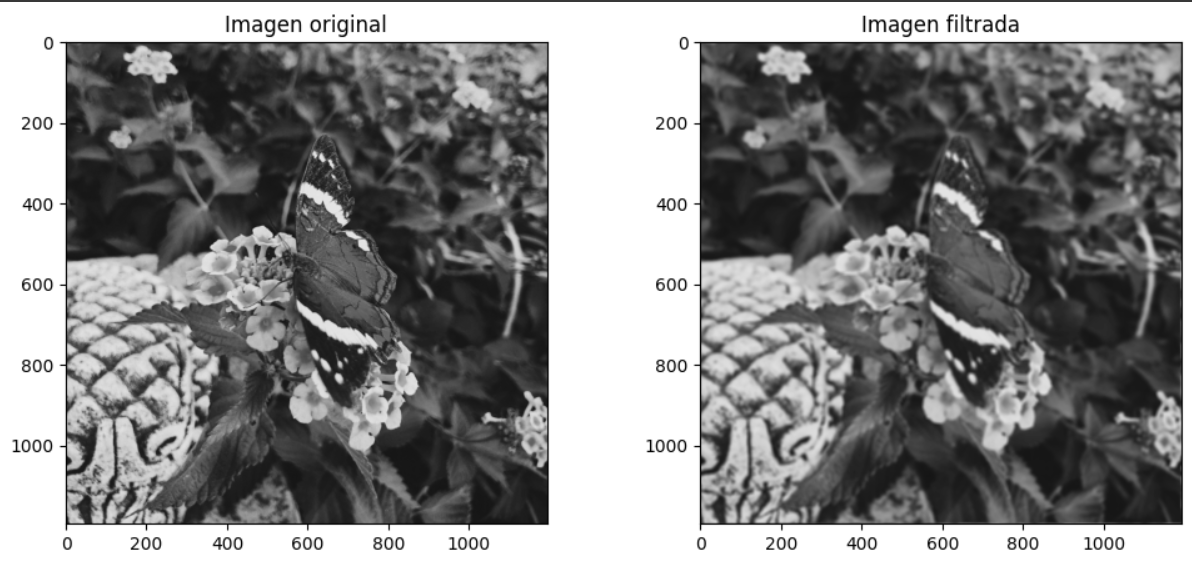
\includegraphics[width=.8\columnwidth]{convolucion.png} 
 \caption{Imagen original (izquierda) contra imagen filtrada (derecha)} \label{fig-1}
\end{figure}

\begin{figure}[!h] 
 \centering
 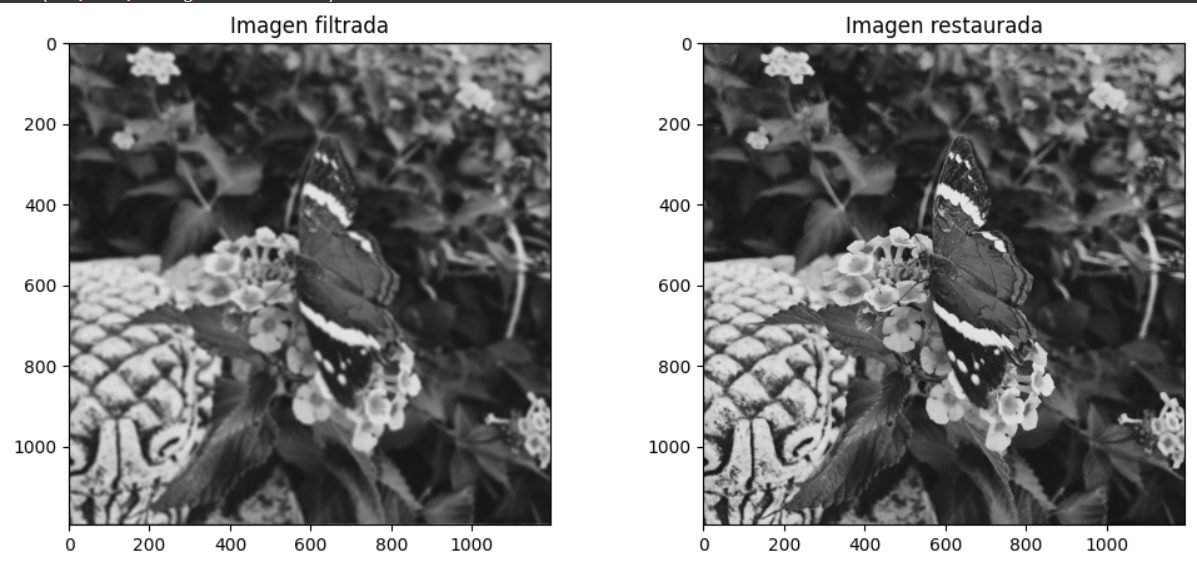
\includegraphics[width=.8\columnwidth]{deconvolucion.png} 
 \caption{Imagen filtrada (izquierda) contra imagen restaurada con filtro inverso (derecha)} \label{fig-1}
\end{figure}
Como podemos observar, la imagen restaurada sale identica a la imagen original ya que usamos el mismo PSF tanto para la convolución como la deconvolución


\bigskip

\textbf{Operador Sobel}

Dentro del procesamiento de imágenes y el computer visión, con el fin de mejorar el reconocimiento de objetos y patrones, se recrea una imagen que contrasta el contorno de los objetos por sobre todo lo demás. Esto se logra a partir de la detección de contornos con el operador Sobel, este consiste en dos kerneles cuya suma de elementos es una matríz de ceros, donde $K_h$ detecta los bordes horizontalmente y $K_v$ verticalemente:

\bigskip 


\begin{equation}
    K_h = 
    \begin{bmatrix}
        -1 & -2 & -1 \\
        0 & 0 & 0 \\
        1 & 2 & 1\\
    \end{bmatrix} 
\end{equation}

\begin{equation}
        K_v = 
    \begin{bmatrix}
        -1 & 0 & 1 \\
        -2 & 0 & -2 \\
        -1 & 0 & 1
    \end{bmatrix}
\end{equation}

Ambas matrices operan cada pixel poniendo el $0$ central por sobre el pixel que buscamos cambiar, si la diferencia de intensidad entre el pixel central y los píxeles colindantes es considerable, el valor resultante de la operación regresará un valor alejado del 0. En cambio, si los píxeles colindantes tiene valores cercanos, el resultado de las dos operaciones con ambas matrices será aproximadamente $0$. Visualmente utilizando UTF-8, esto se traduce en que los contornos de la imagén quedarán de color blanco y el resto será negro.\cite{kim2013applications} Dentro de la restauración de imágenes utilizaremos un proceso basado en el operador Sobel para remarcar los contornos de las imágenes borrosas. 

\textbf {Proceso del código}

Para la resolución del problema se trabajo en base dos metodos. El primero es el... en donde se utiliza una imagen de excelente calidad, la cual se carga en una escala de grises para ajustarla a un tamaño de cuadro. Posteriormente se crea una función para aplicar un filtro gaussiano que tiene como parámetros el kernel de tamaño 5 y una desviación estándar de 1.0, después se utiliza en la imagen convertida en arreglo con los parametros cambiados a 11 y 40 respectivamente, con el fin de que el filtro tenga el mismo tamaño que la imagen. Se utilizaron las funciones "fftn", de la librería scipy.fftpack, la cual calcula la transformada discreta de Fourier con N dimensiones sobre cualquier numero de ejes de un arreglo de M dimensiones mediante la transformada rapida de Fourier (FFT), recibe como parametro un arreglo de entrada. Además de la función "ifftn" que regresa la transformada de Fourier discreta multidimensional inversa, en el código se emplea junto con la función "fftshift" que desplaza el componente de frecuencia cero hacia el centro del espectro, esto con el objetivo de viusalizar la imagen con el desenfoque. 

Por último se aplica en reverso el proceso, se basa en la imagen con desenfoque obtenida. Para esto se divide la transformada de fourier de la imagen desenfocada entre la transformada de Fourier del filtro. A fin de obtener la imagen restaurada se obtiene la transformada inversa de Fourier.

Por otro lado el metodo de deconvolucón ciega, en el cual se parte de una imagen desenfocada se implementó con Matlab. El primer paso es convertir la imagen a escala de grises con el fin de aplicar el procesamiento en dos dimensiones. Después creamos una matríz de unos del tamaño propuesto según nuestra estimación de la PSF. Después utilizamos el método de deconvolución ciega que recibe de parámetros la imagen a deconvolucionar, nuestra suposición incial de la PSF y el número de iteraciones ya que este método se basa en el algorítmo de máxima verosimilitud (MLE). Como el método varía mucho dependiendo de los valores y el tamaño de nuestra PSF inicial, el estandar es iniciar la matríz de uno y probar diferentes tamaños. Después, utilzamos la función edge para detectar los bordes de la figura con  el método de Sobel anteriormente descrito, con la condición de que la intensidad del borde sea mayor a 0.1. Habiendo obtenido los bordes de la imagen, repetimos el proceso con el PSF que estimamos en la primera deconvolución pero considerando más los puntos que caen en los bordes de la figura. El código se encuentra en https://github.com/adara31/Situaci-n-problema

\textbf{}




\section{Análisis de Resultados}
A continuación se presentarán las imágenes que fueron restauradas con deconvolución ciega, así como la PSF estimadas. 

Resultados de imagen de mariposa

\begin{figure}[!h] 
 \centering
 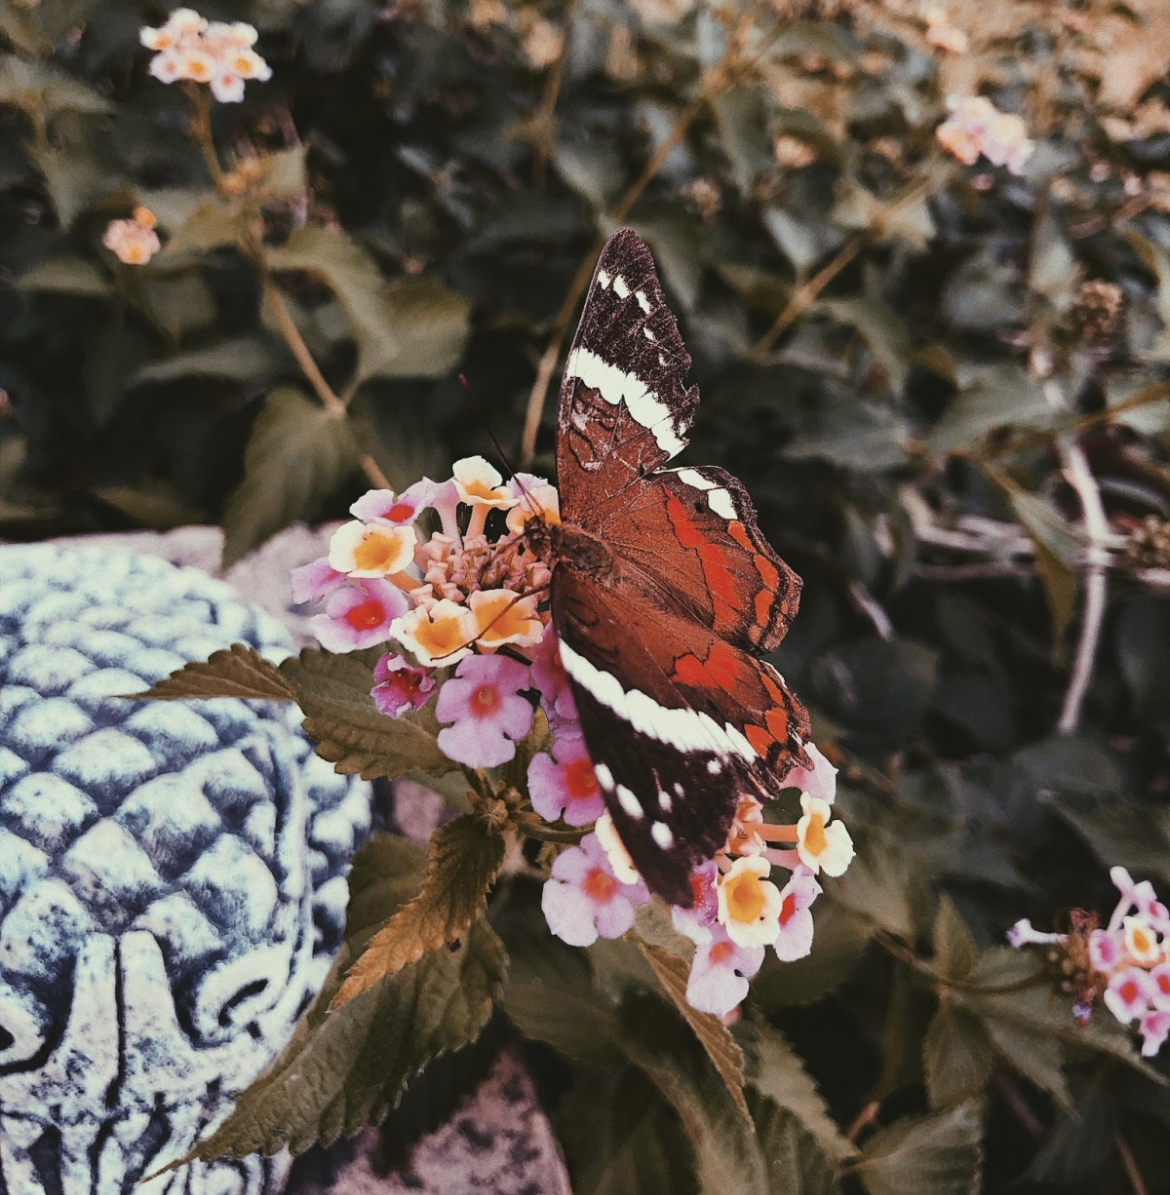
\includegraphics[width=.7\columnwidth]{mariposa.jpeg} 
 \caption{Imagen original de mariposa} \label{fig-1}
\end{figure}

\begin{figure}[!h] 
 \centering
 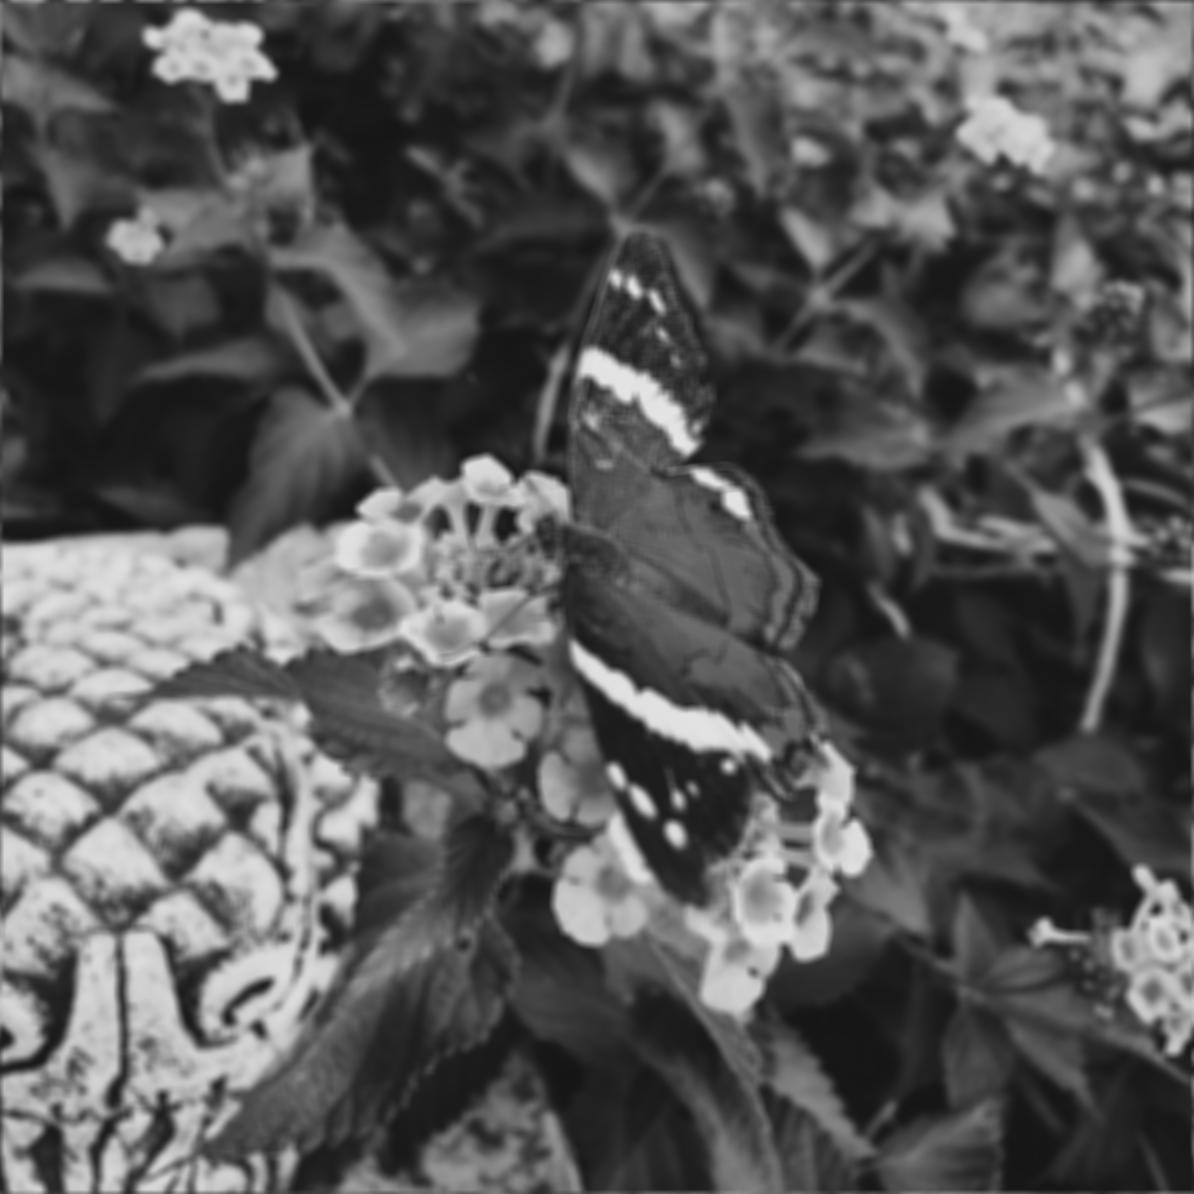
\includegraphics[width=.7\columnwidth]{mariposaBlur.jpeg} 
 \caption{Imagen con filtro Gaussiano aplicado} \label{fig-1}
\end{figure}

\begin{figure}[!h] 
 \centering
 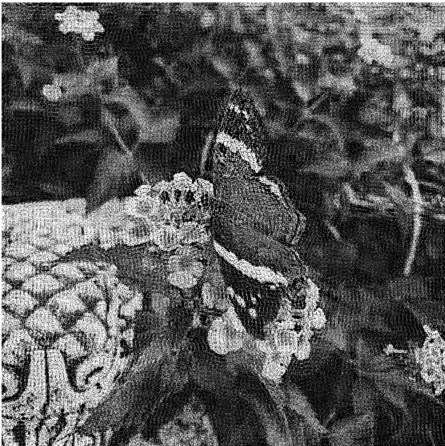
\includegraphics[width=.7\columnwidth]{mariposa_deconv_ciega.png} 
 \caption{Imagen procesada con deconvolución ciega} \label{fig-1}
\end{figure}

Como podemos apreciar en estas imágenes, partimos de una imagen con buena resolución, después el filtro suaviza la imagen. La deconvolución ciega agrega un efecto a la foto, sin embargo los bordes de los objetos y los patrones de la mariposa están evidentemente más definidos. 


Resultados imagen de flores

Si aplicamos un filtro Gaussiano más agresivo en una imagen con buena resuloción, con tamaño del filtro 27 y desviación estandar de 110 obtenemos una imagen más borrosa. Al intentar deconvolucionarla con el proceso ciego, vemos que el resultado no mejora la imagen siginificativamente. 


\begin{figure}[!h] 
 \centering
 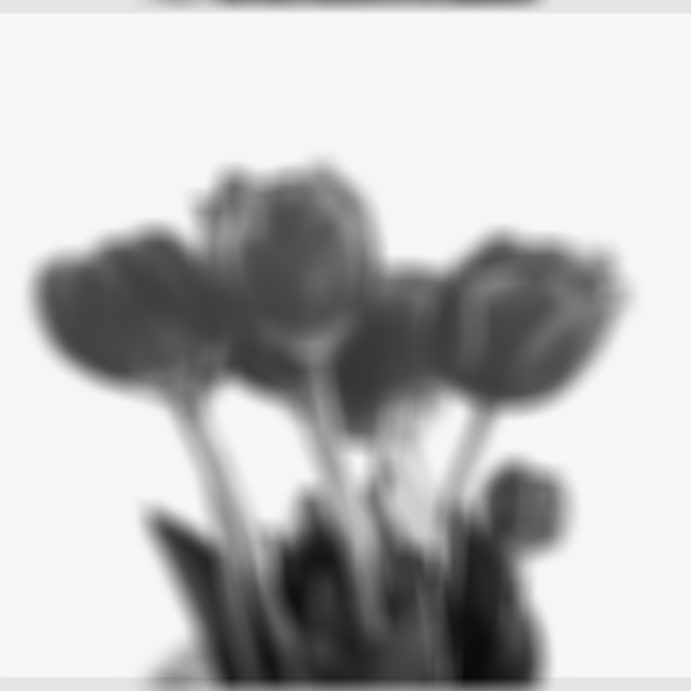
\includegraphics[width=.7\columnwidth]{flores_filtro.png} 
 \caption{Imagen filtrada con filtro Gaussiano agresivo} \label{fig-1}
\end{figure}

\begin{figure}[!h] 
 \centering
 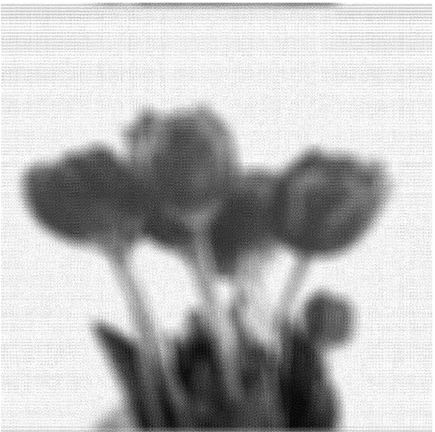
\includegraphics[width=.7\columnwidth]{flores_deconv_blind.png} 
 \caption{Imagen procesada con método de deconvolución ciega} \label{fig-1}
\end{figure}

Para este proceso partimos de una PSF propuesta de tamaño 5x5 de unos. Al finalizar la estimación, la PFS estimada nos da

\begin{equation}
\begin{bmatrix}
       0.039907 & 0.03986 &  0.04013  & 0.0407056\\
   0.040584  &  0.040297   & 0.040743   & 0.040549\\
       0.0398  & 0.0410609 &  0.040037 &  0.040005858\\
   0.0395776   & 0.039411 &  0.03984 &  0.039441 \\
   0.039239  & 0.039160   &0.039380  & 0.0399661\\


\end{bmatrix}
\end{equation}

Si analizamos la estimación del PFS, podemos ver que sí tiene un comportamiento similar al del filtro Gaussiano, donde el valor del centro es más alto que todos los demás, aunado a esto, observamos que lo valores colindantes no varían mucho, esto se esperaría de una vecindad chica del valor central en un filtro con desviación estandar alta como es el caso del filtro orignial. 

\begin{figure}[!h] 
 \centering
 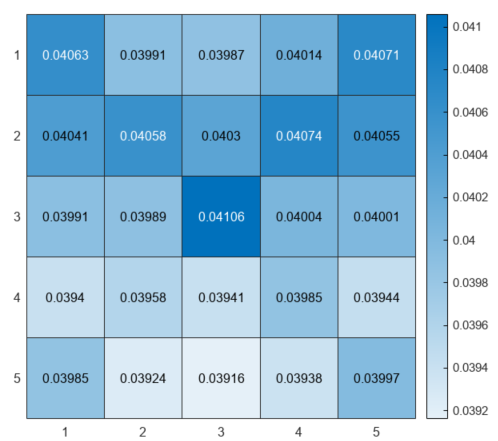
\includegraphics[width=.7\columnwidth]{PSF_estimada.png} 
 \caption{Mapa de calor de la PSF estimada con el método de deconvolución ciega} \label{fig-1}
\end{figure}


En otro experimento, buscamos probar el algoritmo con una imagen proveniente de una dash-cam de baja resolución. 

\begin{figure}[!h] 
 \centering
 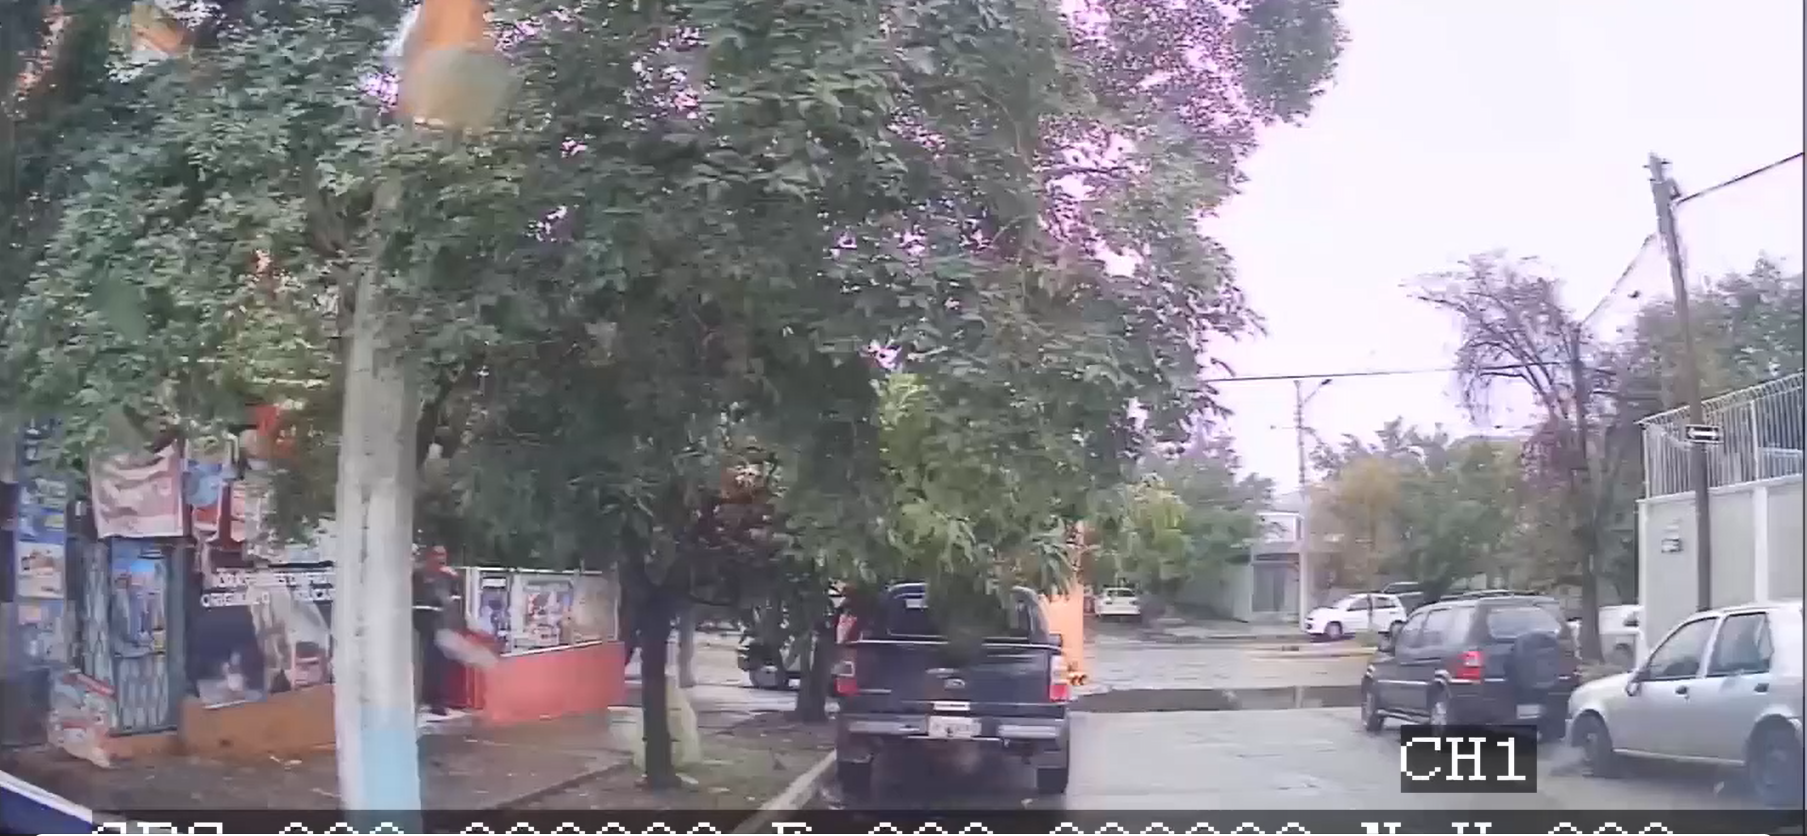
\includegraphics[width=.7\columnwidth]{dashcam_1.png} 
 \caption{Imagen original de dash-cam} \label{fig-1}
\end{figure}

\begin{figure}[!h] 
 \centering
 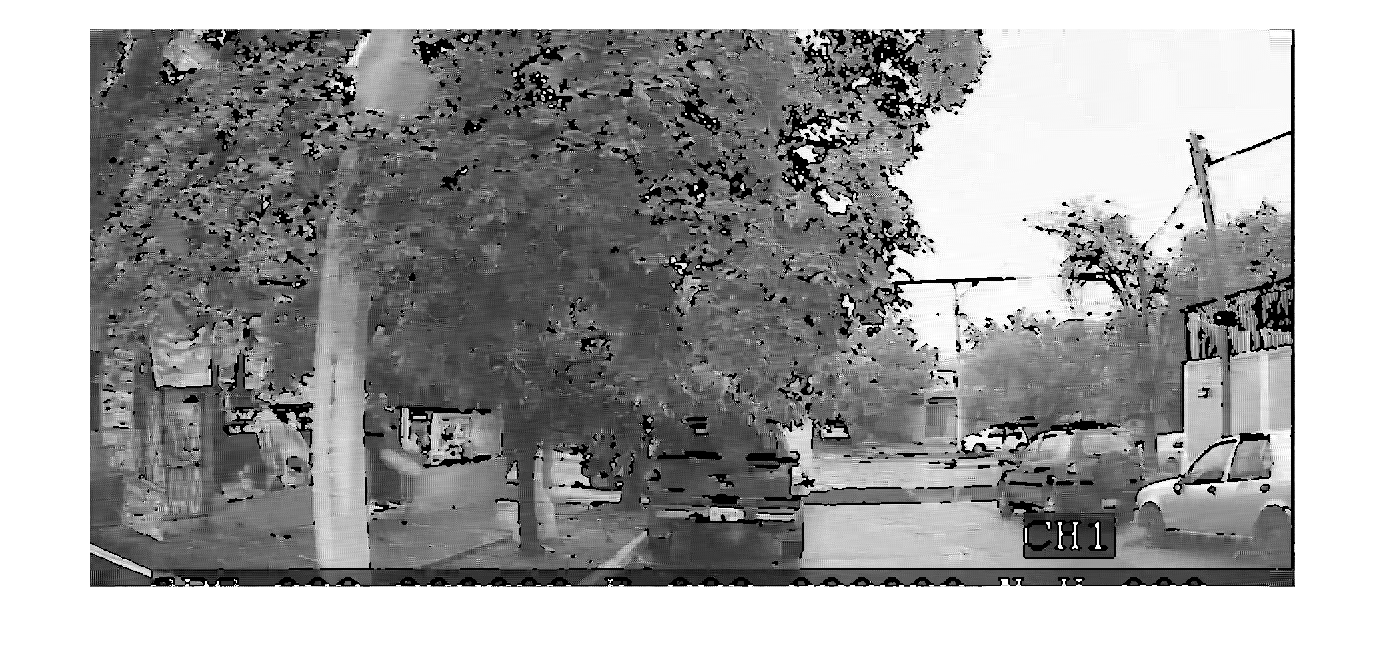
\includegraphics[width=.7\columnwidth]{dahscam_deconv_1.png} 
 \caption{Imagen de dash-cam aplicando la deconvolución ciega} \label{fig-1}
\end{figure}

El resultado de la deconvolución ciega notablemente empeora la imagen, las PSF estimada tmb parece seguir un comportamiento gausiano, sin embargo, los valores son más altos a los de la deconvolución de las flores y hay más diferencia entre los valores de la vecindad. 

\begin{figure}[!h] 
 \centering
 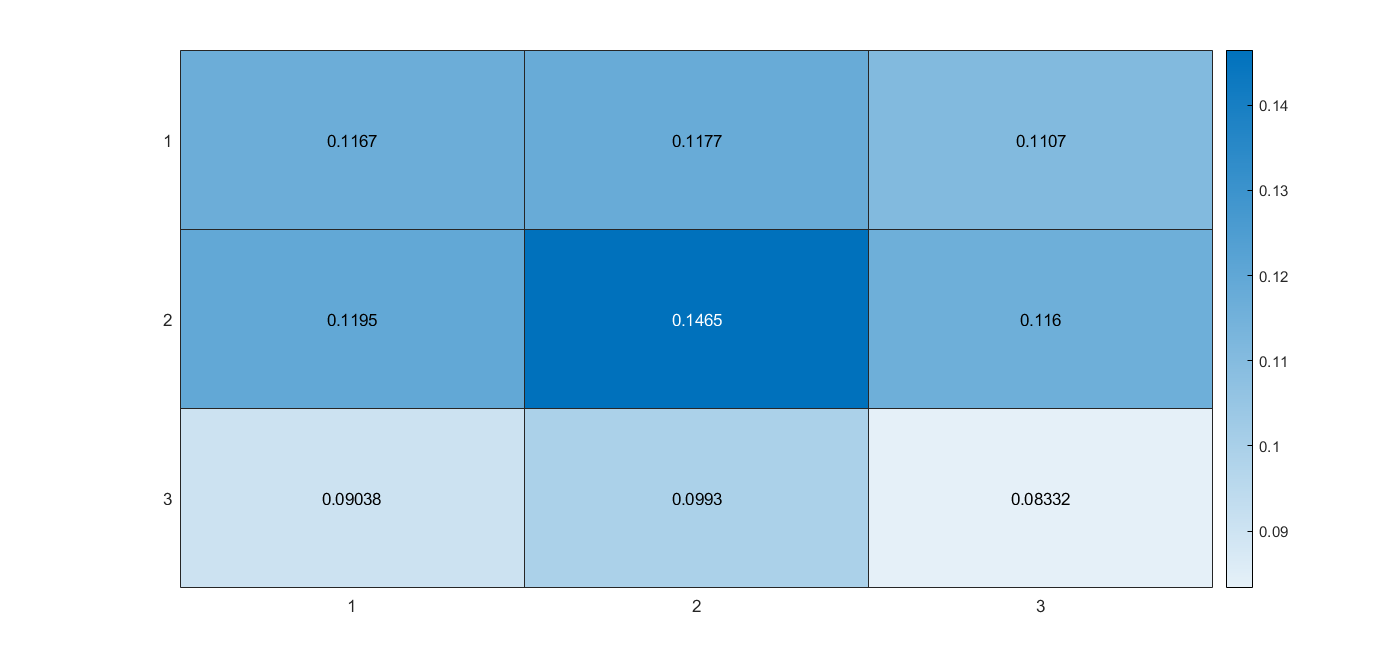
\includegraphics[width=.7\columnwidth]{PSF_estimada_2.png} 
 \caption{Mapa de calor de la PSF estimada con el método de deconvolución ciega} \label{fig-1}
\end{figure}

\bigskip



\section{Conclusiones}

En conclusión este documento ha explorado los metódos de convolución, deconvolución ciega y no ciega, destacando su importante aplicacion en el procesamiento de imagenes. Tras analizar los resultados obtenidos de las imagenes emplementadas se deduce que con un filtro gaussiano de menor tamaño la imagen que se obtiene mediante la deconvolución ciega resulta bien definida de sus bordes, a pesar de producirse un efecto peculiar. Por otro lado, con un filtro gaussiano mayor la imagen restaurada no mejora significativamente la calidad de la imagen, pero la PSF que se produce tiene un comportamiento similar al filtro gaussiano. Por último, en imagenes provinientes de una cámara de baja resolución el resultado del proceso no es aquel deseado. Es importante mencionar que el resultado del método depende en mayor medida de la causa de la degradación de la imagen, para aquellas imagenes que se ven afectadas por el movimiento existen otros métodos más óptimos para su restauración. 

\section{Apéndice}
\url{https://github.com/adara31/Situaci-n-problema}





% Include references
\insertbibliography{References}

\end{document}